% -*- Mode:TeX -*-

%% IMPORTANT: The official thesis specifications are available at:
%%            http://libraries.mit.edu/archives/thesis-specs/
%%
%%            Please verify your thesis' formatting and copyright
%%            assignment before submission.  If you notice any
%%            discrepancies between these templates and the
%%            MIT Libraries' specs, please let us know
%%            by e-mailing thesis@mit.edu

%% The documentclass options along with the pagestyle can be used to generate
%% a technical report, a draft copy, or a regular thesis.  You may need to
%% re-specify the pagestyle after you \include  cover.tex.  For more
%% information, see the first few lines of mitthesis.cls.

%\documentclass[12pt,vi,twoside]{mitthesis}
%%
%%  If you want your thesis copyright to you instead of MIT, use the
%%  ``vi'' option, as above.
%%
%\documentclass[12pt,twoside,leftblank]{mitthesis}
%%
%% If you want blank pages before new chapters to be labelled ``This
%% Page Intentionally Left Blank'', use the ``leftblank'' option, as
%% above.

\documentclass[12pt,twoside]{mitthesis}
\usepackage{lgrind}
\usepackage{url}
%% These have been added at the request of the MIT Libraries, because
%% some PDF conversions mess up the ligatures.  -LB, 1/22/2014
\usepackage{cmap}
%\usepackage{lmodern}
\usepackage{kpfonts}
\usepackage[scaled=.8]{DejaVuSansMono}
\usepackage[T1]{fontenc}
\usepackage{color}
\usepackage{minted}
\usepackage{graphicx}
\usepackage{tcolorbox}
\usepackage{etoolbox}
\BeforeBeginEnvironment{minted}{\begin{tcolorbox}}%
\AfterEndEnvironment{minted}{\end{tcolorbox}}%
\graphicspath{ {images/} }
\pagestyle{plain}

%% This bit allows you to either specify only the fil `p[es which you wish to
%% process, or `all' to process all files which you \include.
%% Krishna Sethuraman (1990).

% \typein [\files]{Enter file names to process, (chap1,chap2 ...), or `all' to
% process all files:}
% \def\all{all}
% \ifx\files\all \typeout{Including all files.} \else \typeout{Including only \files.} \includeonly{\files} \fi

\newcommand{\dr}[1]{{\color{magenta}DR: {#1}}}
\newcommand{\ct}[1]{\texttt{{#1}}}
\newcommand{\libccp}{\ct{libccp}}
\begin{document}

% -*-latex-*-
%
% For questions, comments, concerns or complaints:
% thesis@mit.edu
%
%
% $Log: cover.tex,v $
% Revision 1.8  2008/05/13 15:02:15  jdreed
% Degree month is June, not May.  Added note about prevdegrees.
% Arthur Smith's title updated
%
% Revision 1.7  2001/02/08 18:53:16  boojum
% changed some \newpages to \cleardoublepages
%
% Revision 1.6  1999/10/21 14:49:31  boojum
% changed comment referring to documentstyle
%
% Revision 1.5  1999/10/21 14:39:04  boojum
% *** empty log message ***
%
% Revision 1.4  1997/04/18  17:54:10  othomas
% added page numbers on abstract and cover, and made 1 abstract
% page the default rather than 2.  (anne hunter tells me this
% is the new institute standard.)
%
% Revision 1.4  1997/04/18  17:54:10  othomas
% added page numbers on abstract and cover, and made 1 abstract
% page the default rather than 2.  (anne hunter tells me this
% is the new institute standard.)
%
% Revision 1.3  93/05/17  17:06:29  starflt
% Added acknowledgements section (suggested by tompalka)
%
% Revision 1.2  92/04/22  13:13:13  epeisach
% Fixes for 1991 course 6 requirements
% Phrase "and to grant others the right to do so" has been added to
% permission clause
% Second copy of abstract is not counted as separate pages so numbering works
% out
%
% Revision 1.1  92/04/22  13:08:20  epeisach

% NOTE:
% These templates make an effort to conform to the MIT Thesis specifications,
% however the specifications can change.  We recommend that you verify the
% layout of your title page with your thesis advisor and/or the MIT
% Libraries before printing your final copy.
\title{The Design and Implementation of a Congestion Control Plane}

\author{Akshay Narayan}
%\prevdegrees{S.B., Massachusetts Institute of Technology (2017)}
% If you wish to list your previous degrees on the cover page, use the
% previous degrees command:
%       \prevdegrees{A.A., Harvard University (1985)}
% You can use the \\ command to list multiple previous degrees
%       \prevdegrees{B.S., University of California (1978) \\
%                    S.M., Massachusetts Institute of Technology (1981)}
\department{Department of Electrical Engineering and Computer Science}

% If the thesis is for two degrees simultaneously, list them both
% separated by \and like this:
% \degree{Doctor of Philosophy \and Master of Science}
\degree{Master of Science in Electrical Engineering and Computer Science}

% As of the 2007-08 academic year, valid degree months are September,
% February, or June.  The default is June.
\degreemonth{February}
\degreeyear{2019}
\thesisdate{November 1, 2018}

%% By default, the thesis will be copyrighted to MIT.  If you need to copyright
%% the thesis to yourself, just specify the `vi' documentclass option.  If for
%% some reason you want to exactly specify the copyright notice text, you can
%% use the \copyrightnoticetext command.
%\copyrightnoticetext{\copyright IBM, 1990.  Do not open till Xmas.}

% If there is more than one supervisor, use the \supervisor command
% once for each.
\supervisor{Hari Balakrishnan}{Fujitsu Chair Professor}

% This is the department committee chairman, not the thesis committee
% chairman.  You should replace this with your Department's Committee
% Chairman.
\chairman{Leslie A. Kolodziejski}{Professor of Electrical Engineering and Computer Science\\Chair, Department Committee on Graduate Students}

% Make the titlepage based on the above information.  If you need
% something special and can't use the standard form, you can specify
% the exact text of the titlepage yourself.  Put it in a titlepage
% environment and leave blank lines where you want vertical space.
% The spaces will be adjusted to fill the entire page.  The dotted
% lines for the signatures are made with the \signature command.
\maketitle

% The abstractpage environment sets up everything on the page except
% the text itself.  The title and other header material are put at the
% top of the page, and the supervisors are listed at the bottom.  A
% new page is begun both before and after.  Of course, an abstract may
% be more than one page itself.  If you need more control over the
% format of the page, you can use the abstract environment, which puts
% the word "Abstract" at the beginning and single spaces its text.

%% You can either \input (*not* \include) your abstract file, or you can put
%% the text of the abstract directly between the \begin{abstractpage} and
%% \end{abstractpage} commands.

% First copy: start a new page, and save the page number.
\cleardoublepage
% Uncomment the next line if you do NOT want a page number on your
% abstract and acknowledgments pages.
% \pagestyle{empty}
\setcounter{savepage}{\thepage}
\begin{abstractpage}
This paper describes the implementation and evaluation of a system to implement complex congestion control functions by placing them in a separate agent outside the datapath.  
Each datapath---such as the Linux kernel TCP, UDP-based QUIC, or kernel-bypass transports like mTCP-on-DPDK---summarizes information about packet round-trip times, receptions, losses, and ECN via a well-defined interface to algorithms running in the off-datapath Congestion Control Plane (CCP). 
The algorithms use this information to control the datapath's congestion window or pacing rate. Algorithms written in CCP can run on multiple datapaths. CCP improves both the pace of development and ease of maintenance of congestion control algorithms by providing better, modular abstractions, and supports aggregation capabilities of the Congestion Manager, all with one-time changes to datapaths. 
CCP also enables new capabilities, such as Copa in Linux TCP, several algorithms running on QUIC and mTCP/DPDK, and the use of signal processing algorithms to detect whether cross-traffic is ACK-clocked.
Experiments with our user-level Linux CCP implementation show that CCP algorithms behave similarly to kernel algorithms, and incur modest CPU overhead of a few percent.

\end{abstractpage}

% Additional copy: start a new page, and reset the page number.  This way,
% the second copy of the abstract is not counted as separate pages.
% Uncomment the next 6 lines if you need two copies of the abstract
% page.
% \setcounter{page}{\thesavepage}
% \begin{abstractpage}
% This paper describes the implementation and evaluation of a system to implement complex congestion control functions by placing them in a separate agent outside the datapath.  
Each datapath---such as the Linux kernel TCP, UDP-based QUIC, or kernel-bypass transports like mTCP-on-DPDK---summarizes information about packet round-trip times, receptions, losses, and ECN via a well-defined interface to algorithms running in the off-datapath Congestion Control Plane (CCP). 
The algorithms use this information to control the datapath's congestion window or pacing rate. Algorithms written in CCP can run on multiple datapaths. CCP improves both the pace of development and ease of maintenance of congestion control algorithms by providing better, modular abstractions, and supports aggregation capabilities of the Congestion Manager, all with one-time changes to datapaths. 
CCP also enables new capabilities, such as Copa in Linux TCP, several algorithms running on QUIC and mTCP/DPDK, and the use of signal processing algorithms to detect whether cross-traffic is ACK-clocked.
Experiments with our user-level Linux CCP implementation show that CCP algorithms behave similarly to kernel algorithms, and incur modest CPU overhead of a few percent.

% \end{abstractpage}

\cleardoublepage

\section*{Acknowledgments}
I first thank my advisors for their support and guidance: Hari Balakrishnan and Mohammad Alizadeh, as well as my former advisors, Sylvia Ratnasamy and Scott Shenker.

Second, I thank my CCP colleagues for their ideas, code, feedback, friendship, and support: Frank Cangialosi, Deepti Raghavan, Prateesh Goyal, Srinivas Narayana, and Radhika Mittal.

Third, I thank all the other members of the Networks and Mobile Systems group at MIT CSAIL who have made my time thus far here so enjoyable, especially Anirudh Sivaraman, Ravi Netravali, Amy Ousterhout, Vikram Nathan, Vibhaa Sivaraman, and Venkat Arun.

Fourth, I thank the members of the UC Berkeley Netsys Lab who first taught me how fun research can be, especially Rachit Agarwal, Justine Sherry, Aurojit Panda, Peter Gao, and Gautam Kumar.

Fifth, I thank my friends, especially Sagar Karandikar, Shoumik Palkar, and Paroma Varma for the laughs.

Lastly, and most importantly, I thank my family: Amma, Appa, Madhuri, and Rohan, for all their support.

% -*-latex-*-

% Some departments (e.g. 5) require an additional signature page.  See
% signature.tex for more information and uncomment the following line if
% applicable.
% % -*- Mode:TeX -*-
%
% Some departments (e.g. Chemistry) require an additional cover page
% with signatures of the thesis committee.  Please check with your
% thesis advisor or other appropriate person to determine if such a 
% page is required for your thesis.  
%
% If you choose not to use the "titlepage" environment, a \newpage
% commands, and several \vspace{\fill} commands may be necessary to
% achieve the required spacing.  The \signature command is defined in
% the "mitthesis" class
%
% The following sample appears courtesy of Ben Kaduk <kaduk@mit.edu> and
% was used in his June 2012 doctoral thesis in Chemistry. 

\begin{titlepage}
\begin{large}
This doctoral thesis has been examined by a Committee of the Department
of Chemistry as follows:

\signature{Professor Jianshu Cao}{Chairman, Thesis Committee \\
   Professor of Chemistry}

\signature{Professor Troy Van Voorhis}{Thesis Supervisor \\
   Associate Professor of Chemistry}

\signature{Professor Robert W. Field}{Member, Thesis Committee \\
   Haslam and Dewey Professor of Chemistry}
\end{large}
\end{titlepage}


\pagestyle{plain}
  % -*- Mode:TeX -*-
%% This file simply contains the commands that actually generate the table of
%% contents and lists of figures and tables.  You can omit any or all of
%% these files by simply taking out the appropriate command.  For more
%% information on these files, see appendix C.3.3 of the LaTeX manual. 
\tableofcontents
\newpage
\listoffigures
\newpage
\listoftables


\chapter{Introduction}
Research on congestion control has not only remained vibrant since the 1980s, but has flourished in recent years as new applications, network technologies, and workload patterns have been emerging at a rapid rate. Figure~\ref{fig:cctimeline} shows a time-line of innovations in this area.

At its core, a congestion control protocol determines when each segment of data must be sent. Because a natural place to make this decision is within the transport layer, congestion control today is tightly woven into kernel TCP software and runs independently for each TCP connection.

This design has three shortcomings. First, many modern proposals use techniques such as Bayesian forecasts (Sprout~\cite{sprout}), offline or online learning (Remy~\cite{remy}, PCC~\cite{pcc}, PCC-Vivace~\cite{pcc-vivace}, Indigo~\cite{pantheon}), or signal processing with Fourier transforms (Nimbus~\cite{nimbus}) that are difficult, if not impossible, to implement in a kernel lacking useful libraries for the required calculations. For example, computing the cube root function in Linux's Cubic implementation requires using a table lookup and a Newton-Raphson iteration instead of a simple function call. Moreover, to meet tight performance constraints, in-kernel congestion control methods have largely been restricted to simple window or rate arithmetic.

%However, this tight coupling is not fundamental to congestion control; rather,
%it imposes an artificial restriction on algorithms to restrict their
%computations to a single packet inter-arrival time lest they slow down the
%flow.
%Research on congestion control is flourishing, and newly proposed algorithms lacking kernel %implementations, such as
%PCC-Vivace~\cite{pcc-vivace}, Nimbus~\cite{nimbus}, Remy~\cite{remy}, and
%Sprout~\cite{sprout}, 
%all involve calculations that are cumbersome to perform in
%he kernel and challenging to engineer to meet tight performance
%requirements.
%For example, Nimbus uses Fast Fourier Transforms to determine the amount and
%nature of the cross-traffic on the bottleneck link.

Second, the kernel TCP stack is but one example of a {\em datapath}, the term we use for any module that provides data transmission and reception interfaces between higher-layer applications and lower-layer network hardware. Recently, new datapaths have emerged, including user-space protocols atop UDP (e.g., QUIC~\cite{quic}, WebRTC~\cite{webrtc}, Mosh~\cite{mosh}), kernel-bypass methods (e.g., mTCP/DPDK~\cite{dpdk,mtcp,netmap}), RDMA~\cite{dcqcn}, multi-path TCP (MPTCP)~\cite{mptcp}, and specialized Network Interface Cards (``SmartNICs''~\cite{smartnic}). This trend suggests that future applications will use datapaths different from traditional kernel-supported TCP connections.

\begin{figure}[t]
\centering
    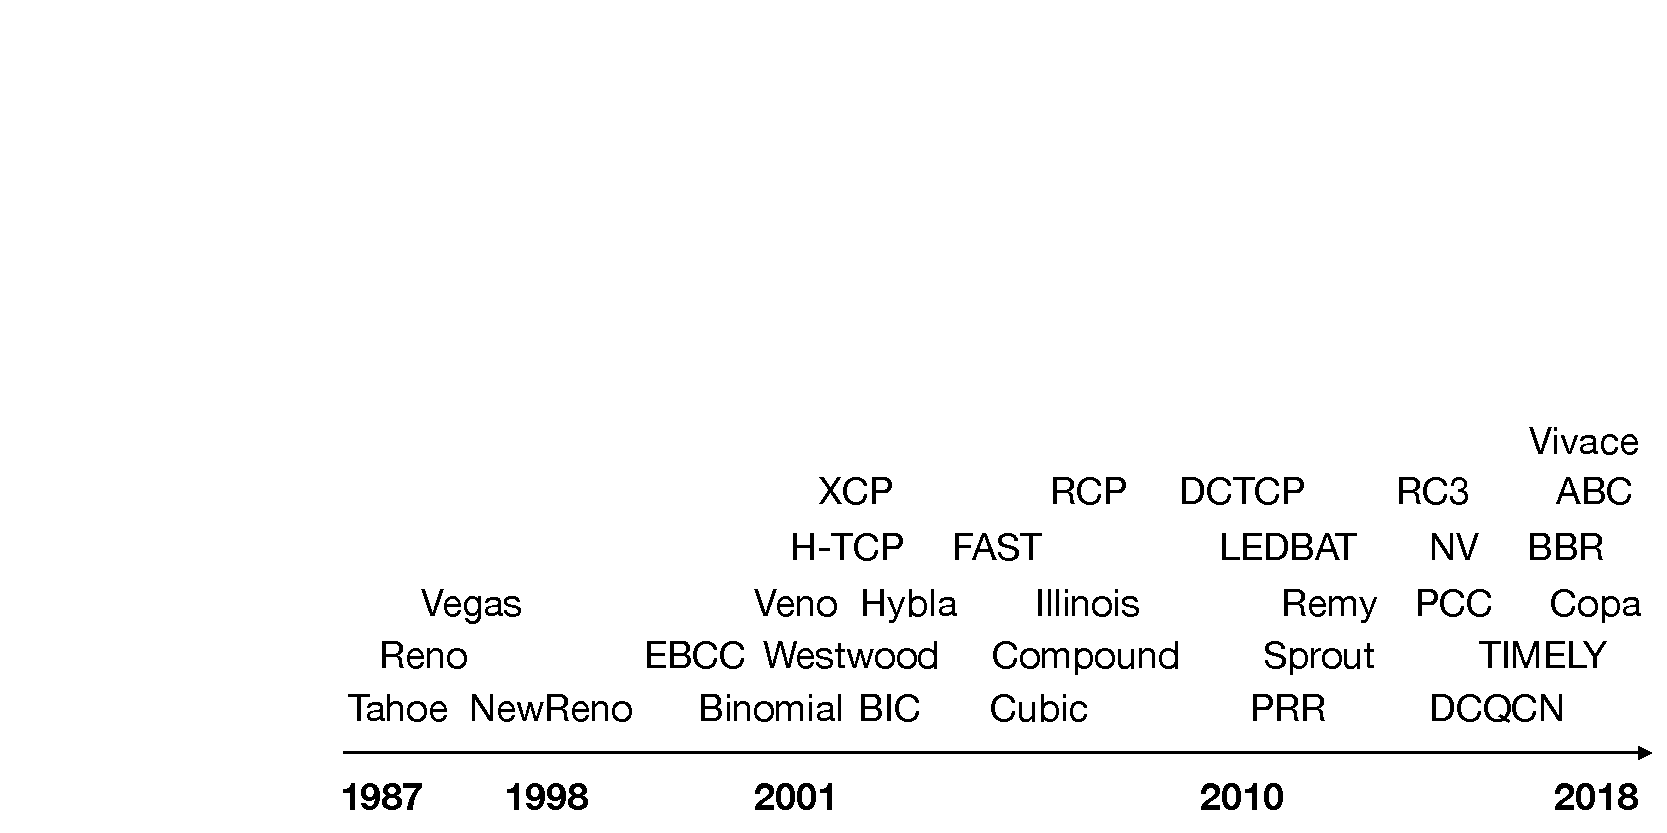
\includegraphics[width=\columnwidth]{img/cc-timeline-nocongsig}
    %\vspace{-20pt}
    %\caption{Congestion control algorithms over the years.}
    \caption{As link characteristics diversify, developers have developed a battery of congestion control algorithms, from the ``long-fat pipe'' schemes of the mid-2000s~\cite{westwood, veno, htcp, hybla} to purely delay-based~\cite{vegas, fasttcp, ledbat, nv, timely} and hybrid loss-delay~\cite{illinois, compound} schemes, and more recent proposals~\cite{pcc, remy, sprout, bbr, copa, abc}.}\label{fig:cctimeline}
    %\vspace{-16pt}
\end{figure}

New datapaths offer limited choices for congestion control because implementing these algorithms correctly takes considerable time and effort. 
We believe this significantly hinders experimentation and innovation both in the datapaths and the congestion control algorithms running over them.
For instance, the set of currently available algorithms in mTCP~\cite{mtcp}, a TCP implementation on DPDK, is limited to a variant of Reno. 
QUIC, despite Google's imposing engineering resources, does not have implementations of several algorithms that have existed in the Linux kernel for many years.  
We expect this situation to worsen with the emergence of new hardware accelerators and programmable network interface cards (NICs) because high-speed hardware designers tend to forego programming convenience for performance. 
%The difficulty is not the volume of code, but rather is the subtle correctness and performance issues in various algorithms that require expertise to understand and resolve.

Third, tying congestion control tightly to the datapath makes it hard to provide new capabilities, such as aggregating congestion information across flows that share common bottlenecks, as proposed in the Congestion Manager project~\cite{cm}. 

%This paper starts from the observation that congestion control algorithms need not be implemented in the datapath. 

\smallskip
If, instead, the datapath encapsulated the information available to it about {\em congestion signals} like packet round-trip times (RTT), receptions, losses, ECN, etc., and periodically provided this information to an off-datapath module, then congestion control algorithms could run in the context of that module. 
By exposing an analogous interface to control transmission parameters such as the window size, pacing rate, and transmission pattern, the datapath could transmit data according to the policies specified by the off-datapath congestion control algorithm. Of course, the datapath must be modified to expose
such an interface, but this effort needs to be undertaken only once for each datapath.
%, and does not grow with the number of congestion control algorithms.

We use the term {\em Congestion Control Plane (CCP)} to refer to this off-datapath module. Running congestion control in the CCP offers the following benefits:
\begin{enumerate}
    \item {\bf Write-once, run-anywhere:} One can write a congestion control algorithm once and run it on any datapath that supports the specified interface. 
    We describe several algorithms running on three datapaths: the Linux kernel, mTCP/DPDK, and QUIC, and show algorithms running for the first time on certain datapaths (e.g., Cubic on mTCP/DPDK and Copa on QUIC).
    \item {\bf Higher pace of development:} With good abstractions,
      a congestion control designer can focus on the algorithmic essentials
      without worrying about the details and data structures of the
      datapath. The resulting code is easier to read and maintain. In our implementation, congestion control algorithms in CCP are written in Rust or Python and run in user space. 
    \item {\bf New capabilities:} CCP makes it easier to provide new
      capabilities, such as aggregate control of multiple flows~\cite{cm}, and algorithms that require sophisticated computation (e.g., signal processing, machine learning, \etc) running in \userspace programming environments. 
      %These algorithms are hard to write as window updates on incoming ACKs.
      %All the benefits of a \userspace programming environment (libraries, debuggers, \etc) will be available to       developers.
\end{enumerate}

%\vspace{0.1in}
\smallskip 
This paper's contributions include:

\begin{itemize}
\item An event-driven language to specify congestion control
  algorithms. Algorithm developers specify congestion control behavior using
  combinations of events and conditions, such as the receipt of an
  ACK or a loss event, along with corresponding handlers to perform
  simple computations directly in the datapath (\eg increment the window) or defer
  complex logic to a \userspace component. We show how to implement several recently proposed algorithms and also congestion-manager aggregation. 

\item A specification of datapath responsibilities. These include congestion
  signals that a datapath should maintain (Table~\ref{tab:api}), as
  well as a simple framework to execute directives from a CCP program. This
  design enables ``write-once, run-anywhere'' protocols.

%\item A demonstration of new capabilities enabled by CCP, including
%   new congestion control algorithms and the implementation of an
%  aggregate congestion controller acting on behalf of multiple flows.

\item An evaluation of the fidelity of CCP relative to in-kernel
  implementations under a variety of link conditions. Our CCP implementation
  matches the performance of Linux kernel implementations at only a small
  overhead (5\% higher CPU utilization in the worst case).
%  Furthermore, we show it  is feasible to implement infrequent congestion control even in low-RTT, high
  % bandwidth environments.

\end{itemize}

\chapter{Related Work}
Congestion control has been an active area of research since the 1980s.
This section both discusses various congestion control algorithms, as well as current pluggable congestion control interfaces present in both QUIC and the Linux Kernel.
Finally, we discuss the CCP userspace agent, which 
\section{Congestion Control}

\section{QUIC}

\section{CCP}
CCP userspace module blah blah blah

\chapter{Implementation: Designing CCP Datapaths}
The advantage of the CCP system includes allowing algorithm developers to not concern themselves with deploying their code on different datapaths.
A CCP compatible datapath needs to accurately enforce the congestion control algorithm sent down by the CCP userspace module. Algorithm developers do not need to worry about datapath specific concerns, such as accurately measuring signals and setting the correct sending rate. Furthermore, once a datapath correctly implements support for CCP, this automatically enables support for all CCP algorithms.

In order to implement support for CCP in both QUIC and the Linux Kernel, we designed a CCP datapath API, \libccp, to make the life of the datapath developer easier. This API clearly defines the job of the datapath developer as well as handles CCP specific computation common to all datapaths. This chapter briefly describes the CCP algorithm interface, and then it describes the implementation of \libccp, and how we use \libccp to design a CCP datapath in QUIC.

\section{CCP Algorithm Interface}
At a high level, congestion control algorithms measure and update statistics about the network, every time they receive new information, usually on packet ACK arrivals, in order to decide how fast to send packets. TCP, for example, in its normal operation, keeps increasing the congestion window until seeing a packet loss, upon which it cuts the congestion window in half.
All CCP datapaths must work with the CCP Agent, run in userspace on the same host.
To support the CCP algorithms written, datapaths must calculate aggregate measurements written over certain congestion primitives, and perform actions at the correct time. These actions include setting windows and pacing rates, as well as reporting measurements back up the main CCP agent.
In the Linux kernel, and in QUIC, congestion control decisions are tied to the ACK clock - decisions must be made everytime an ACK arrives, signaling a congestion event.
Another advantage of CCP is that algorithms can take congestion control actions off of the ACK clock, by explicitly defining a slow path and a fast path program.
In the slow path program, written through the CCP API, algorithms respond to reports that are sent up at granularities specified by the fast path.
Fast path programs run in the datapath, per ACK, and send reports up for the slow path programs to respond to.
The CCP API is currently written in Rust, with bindings to Python.  must write two functions in the slow path:
  \begin{itemize}
    \item \texttt{onCreate} - what to do when a flow is created. Users must install some program here, or else they will not get any measurements
    \item \texttt{onReport} - what to do with measurements when reports are received. This may involve some more complicated calculation, such as fast fourier transforms or neural networks.
  \end{itemize}

\subsection{Fast path programs}
Installing a program involves sending down a string, that defines variables, event handlers. These programs use a Scheme-like syntax The variables are aggregated measurements over certain congestion primitives provided by the datapath. The event handlers consist of a condition, and instructions to execute if the condition is true. Event conditions can access the user defined variables, or other special variables, such as time.
Below is an excerpt of the CCP BBR program sent down to the datapath.

%{\footnotesize
\begin{minted}{lisp}
(def
    (acked 0)
    (lost  0)
)
(when true
    (:= acked (+ acked Ack.bytes_acked))
    (:= lost  (+ lost  Ack.lost_pkts_sample))
    (fallthrough)
)
(when (> lost 0)
    (report)
)
\end{minted}

Table~\ref{tab:api} define the operations, primitive congestion signals, and variable scopes supported by the CCP.
\begin{table}
    \label{tab:api}
    \centering
    \begin{tabular}{p{0.35\columnwidth}p{0.5\columnwidth}}
        \hline
        \hline
        \multicolumn{2}{c}{Primitive congestion signals} \\
        \hline
        \hline
        \textbf{Signal} & \textbf{Definition} \\
        \texttt{Ack.bytes\_acked}, \texttt{Ack.packets\_acked} & In-order acknowledged \\
        \texttt{Ack.bytes\_misordered}, \texttt{Ack.packets\_misordered} & Out-of-order acknowledged \\
        \texttt{Ack.ecn\_bytes}, \texttt{Ack.ecn\_packets} & ECN-marked \\
        \texttt{Ack.lost\_pkts\_sample} & Number of lost packets \\
        \texttt{Ack.now} & Datapath time (e.g., wall clock time)\\
        \texttt{Flow.was\_timeout} & Did a timeout occur? \\
        \texttt{Flow.rtt\_sample\_us} & A recent sample RTT \\
        \texttt{Flow.rate\_outgoing} & Outgoing sending rate \\
        \texttt{Flow.rate\_incoming} & Receiver-side receiving rate  \\
        \texttt{Flow.bytes\_in\_flight}, \texttt{Flow.packets\_in\_flight} & Sent but not yet acknowledged \\
        & \\
        \hline
        \hline
        \multicolumn{2}{c}{Operators} \\
        \hline
        \hline
        \textbf{Class} & \textbf{Operations} \\
        Arithmetic & $+, -, *,$~/$,$ EWMA \\
        Assignment & $:=$ \\
        Comparison & $==, <, >$, or, and \\
        Conditionals & If (branching) \\
        & \\
        \hline
        \hline
        \multicolumn{2}{c}{Variable Scopes} \\
        \hline
        \hline
        \textbf{Scope} & \textbf{Description} \\
        \texttt{Ack} & Signals measured per packet \\
        \texttt{Flow} & Signals measured per connection \\
        \texttt{Timer} & Multi-resolution timer that can be zeroed by a call to \texttt{reset} \\
    \end{tabular}
    %\vspace{0.075in}
    \caption{Fast path language: primitive signals, operators, and scopes. As per the CCP API, datapaths must exposes these signals and operators}
\end{table}


\section{Responsibilities of a CCP Datapath}

A CCP datapath must parse and run a program sent down by the CCP agent that represents a congestion control algorithm.
In order to do this accurately, a CCP datapath has three main responsibilities.
  \begin{itemize}
    \item Establish an IPC mechanism.
    \item Correctly enforce congestion windows and pacing rates
    \item Accurately measure the variables defined, and run the program sent by the user everytime new information comes.
  \end{itemize}
First, it must communicate with the CCP agent, that runs on the same host, using some interprocess communication (IPC) mechanism.
The current implementation of the CCP Agent expects that the datapath communicates through a single persistent connection.
Regardless of how many new flows enter, the datapath must be able to send and receive messages about all flows over this single connection.
It must assign flow IDs and uses these IDs to distinguish between flows when serializing and deserializing messages.

In order to accurately enforce the sending patterns of the congestion control algorithm, datapaths should enforce pacing rates and congestion windows separately. This would allow an algorithm to specify a congestion window with a rate cap, in order to prevent bursty transmission.

Third, the datapath must measure congestion signals accurately and report them to the CCP agent at the specified timing patterns.
This involves correctly installing and performing the programs sent down by the CCP agent, which specify how to aggregate and report measurements over the congestion primitives and how to set the congestion window and pacing rate. While the CCP agents turns the user's programs into a serialized set of instructions for the datapath, the datapath must ensure safe execution of the instructions. For the Linux kernel datapath, this involves ensuring that instructions cannot cause a divide by zero that would crash the kernel.


\section{Libccp}

To help add CCP support in various datapaths, we created a shared library in C, named \libccp that provides a reference implementation for the features common to all CCP datapaths: serialization of messages and execution of the program sent down by the userspace agent.
As we built our kernel, QUIC, and mTCP datapaths simultaneously, having one body of shared code prevented reimplementing the same work to multiple datapaths.
This shared library also reduces the responsibilities required by CCP datapaths to provide support for CCP algorithms.
Now datapath developers solely need to focus on (i) \textit{correctly defining primitive congestion signals} and (ii) \textit{correctly exposing mechanisms to set congestion windows and pacing rates}
Specifically, to implement the datapath API, datapaths must provide a set of function pointers, set up IPC with some form compatible with userspace CCP (character device or netlink sockets for kernel datapaths, and unix sockets for userspace datapaths), and fill in the congestion signal primitives everytime new information arrives.
Datpath developers must provide function pointers that do the following:
\begin{enumerate}
    \item Set a congestion window (in bytes)  or pacing rate (either an absolute rate, or relative to current rate) given a flow ID
    \item Provide a notion of time: now, since, and after (in microseconds)
    \item Send a message through the IPC to the userspace CCP agent
\end{enumerate}
Each of these functions takes in a pointer to \ct{struct ccp\_connection}, which contains information for this flow. \ct{ccp\_connection} includes one field for datapath specific state per flow. In the Linux kernel, for example, this is pointer to the \ct{tp\_sock} object, to access congestion state for the correct connection.

In return, \libccp provides two functions that the datapath can call to make userspace CCP algorithms work properly.
\begin{itemize}
    \item \texttt{ccp\_invoke}: After updating the primitive congestion signals on ACKs and timeouts, \texttt{ccp\_invoke} will invoke the program state machine stored inside \libccp. This will run through all of the events in the currently installed program, ending with an optional report to the userspace CCP agent; the events will automatically invoke the function pointers that set the rate or cwnd within the datapath.
    \item \texttt{ccp\_read\_msg}: Upon reading a message from the IPC mechanism, the datapath can call \texttt{ccp\_read\_msg}. 
        Currently, CCP can send down two types of messages: a message that updates the value of a particular variable defined by the fast past program, or a message to install a new fast path program completely. 
        \libccp will deserialize the message to parse both the flow ID and message type from the header, in order to perform the correct update for the correct flow.
\end{itemize}

With the architecture of the \libccp API, adding support into QUIC for supporting CCP was relatively easy.

\section{Current Congestion Control Architecture in QUIC}
As discussed in \dr{related work}, the QUIC already supports pluggable congestion control in userspace. \dr{ref to send algorithm interface}
\begin{figure}[h]
\centering
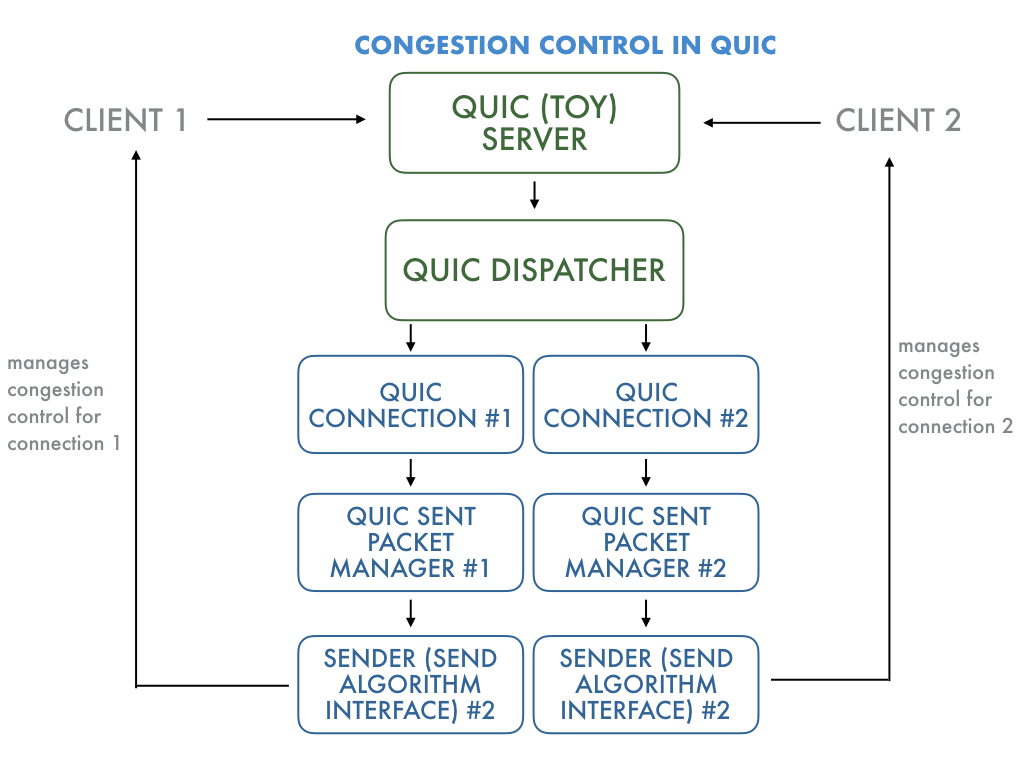
\includegraphics[scale=.45]{implementation/quiccc}
\caption{In QUIC, when the toy server sees a client request, the \ct{SimpleDispatcher} object spawns a new \ct{QuicConnection} object that handles the connection. To manage sending packets, the \ct{QuicConnection} object creates a \ct{QuicSentPacketManager}. The \ct{QuicSentPacketManager} creates a \ct{Sender} object that uses the function callbacks from the \ct{SendAlgorithmInterface} specified as the current congestion control setting.}
\label{fig:quiccc_diagram}
\end{figure}

As Fig~\ref{fig:quiccc_diagram} shows, QUIC uses the \ct{SendAlgorithmInterface} class to allow developers to add in new algorithms.
The \ct{SendAlgorithmInterface} contains most of the features necessary to support a CCP datapath.
The \ct{GetCongestionWindow()} and \ct{PacingRate()} functions allow algorithms to set particular congestion windows and pacing rate.
Pacing is implemented through a separate sender class with a typical token bucket scheme. When deciding whether to send more, the \ct{QuicConnection} object invokes the \ct{CanSend} callback.
This function takes in the number of bytes in flight, and checks whether the congestion window is less, so the sender can send more.
If pacing is enabled and the pacing rate is not 0, the \ct{QuicConnection} checks whether sending should be delayed due to pacing.
Three functions allow senders to measure the congestion signals specified in Table~\ref{tab:api}:
\begin{itemize}
	\item \ct{OnCongestionEvent}: Incoming ACKs or loss event timeouts trigger this function, which provides a vector of acked packets, a vector of lost packets, a boolean indicating if the RTT has been updated, and the prior in flight byte count.
	\item \ct{OnPacketSent}: This callback provides new information on the current number of bytes in flight.
	\item \ct{OnRetransmissionTimeout}: This callback allows senders to take any special actions in the case of timeouts; packets are not counted as lost in the case of timeouts.
\end{itemize}

To implement support for CCP, it is not enough to just implement a sender.
The main requirement for off datapath congestion control is the ability to use an IPC mechanism to communicate between the in datapath sender and the off datapath congestion control.
Each sender object could independently spawn an IPC mechanism and communicate with the CCP agent, but the current implementation does not support this.
As QUIC is another userspace process, each sender could use UDP to communicate with CCP.
However, the current design of CCP requires that the datapath has one persistent connection with the CCP agent, where messages are received and sent regarding all current flows.
Since each sender is an independent object, it only knows about its own flow; some object higher in the hierarchy from Figure~\ref{fig:quiccc_diagram} must control IPC with the CCP agent.

\section{Implementing Libccp API in QUIC}
\subsection{Architecture}
\begin{figure}[h]
\centering
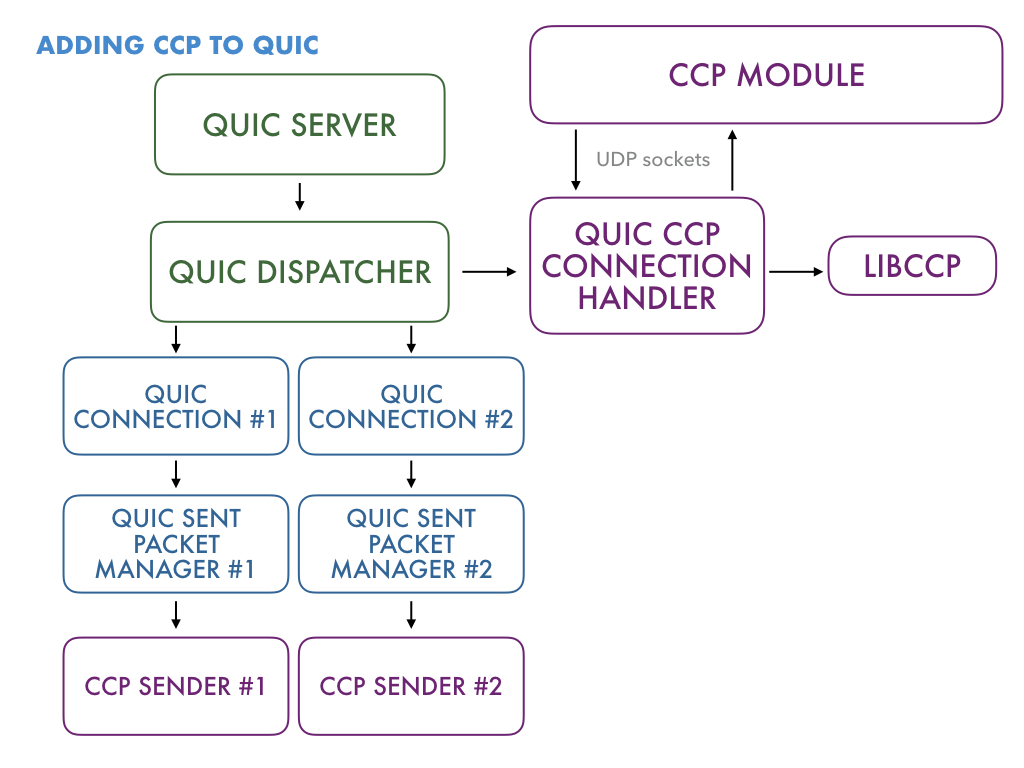
\includegraphics[scale=.45]{implementation/ccpquic_diagram}
\caption{The \ct{QuicCCPConnectionHandler} class implements the \libccp API. It provides the time related functions through the C++ standard library's wall clock time. By passing in the pointer to the specific \ct{QuicConnection} object to a call to \ct{Set\_Congestion\_Window}, the CCP connection handler propagates the instruction down to the specific CCP sender object.}
\label{fig:ccpquic_diagram}
\end{figure}


To implement CCP support in QUIC, we add a new \ct{CCPSender} class that implements the \ct{SendAlgorithmInterface}.
To handle IPC communication with the CCP Agent, we create a new object, the \ct{CCPConnectionHandler}, that uses UDP sockets.
In addition, all the function pointers required by the \libccp API are provided through this class.
The \ct{SimpleDispatcher} owns the \ct{CCPConnectionHandler}; Figure~\ref{fig:ccpquic_diagram} details how the new classes fit into the overall QUIC congestion control architecture.
Upon starting a new connection, the connection handler sets up CCP related state for the flow.
It saves a pointer to the \ct{QuicConnection} object in the \libccp state for this flow.
Later when the fast path program is running and \libccp must set a window or pacing rate for this flow, \libccp calls the set window pointer in the \ct{CCPConnectionHandler} with the \ct{QuicConnection} pointer as argument.

\subsection{Congestion Signal Measurement}\
\begin{table}
    \label{tab:quicsignaldef}
    \centering
    \begin{tabular}{p{0.35\columnwidth}p{0.5\columnwidth}}
        \hline
        \hline
        \multicolumn{2}{c}{Primitive congestion signals} \\
        \hline
        \hline
        \textbf{Signal} & \textbf{Definition} \\
        \texttt{Ack.bytes\_acked}, \texttt{Ack.packets\_acked} & Number of bytes received in order in a call to \ct{OnCongestionEvent} before the first lost packet, from the \ct{AckedPackets} vector passed in as an argument \\
        \texttt{Ack.bytes\_misordered}, \texttt{Ack.packets\_misordered} & Number of bytes received in the \ct{AckedPackets} vector with a sequence number greater than the sequence number of the first lost packet. \\
        \texttt{Ack.lost\_pkts\_sample} & Number of lost packets, i.e. size of the \ct{LostPackets} passed into the \ct{OnCongestionEvent} function. \\
        \texttt{Ack.now} & C++ Standard library wall clock time\\
        \texttt{Flow.was\_timeout} & True when \ct{OnRetransmissionTimeout} is called \\
        \texttt{Flow.rtt\_sample\_us} & The most recent new RTT sample.\\
        \texttt{Flow.rate\_outgoing} & Outgoing sending rate \\
        \texttt{Flow.rate\_incoming} & Receiver-side receiving rate, measured at the sender.  \\
        \texttt{Flow.bytes\_in\_flight}, \texttt{Flow.packets\_in\_flight} & Updated whenever a packet is sent for a new estimate of the number of bytes currently in the pipe. \\
    \end{tabular}
    %\vspace{0.075in}
    \caption{On ACKs, the \ct{CCPSender} uses these definitions to update the calculations of the primitive congestion signals}
\end{table}

Each sender individually measures congestion signals, and calls \ct{ccp\_invoke} to trigger execution of the fastpath program within \libccp.
Table~\ref{tab:quicsignaldef} specifies, within QUIC, how each congestion signal is calculated.
QUIC's notion of acknolwedgements is different from the Linux kernel. The Linux kernel uses the notion of ``sack'' to indicate a packet is lost.
The sender will see acknowledgements for the 3 sequence numbers after the lost packet.
In contrast, QUIC keeps a map of bytes in flight and can explicitly provide information about which sequence numbers are lost, within a block of packets.
\dr{explain this better; explain loss recovery in QUIC better}

\section{Summary of Implementation}
We implement CCP support in the QUIC Toy Server, in the publicly released chromium code base.
The changes, in total, include:
\begin{itemize}
    \item New \ct{CCPSender} that implements the send algorithm interface
    \item Modify \ct{QuicConnection} and \ct{QuicSentPacketManager} classes to allow setting windows for the underlying \ct{CCPSender}
    \item New \ct{QuicCCPConnectionHandler} class
    \item Modify \ct{QuicSimpleDispatcher}, used by the toy server, to spawn a connection handler when starting a new connection
    \item Add \ct{libccp} as a third party library
    \item Command line options when running the toy server to control which congestion control option is set
    \item New congestion window logger class to help with experimenting
\end{itemize}
All the changes are based on top of Chromium commit hash \textbf{dedfa29047}, and comprise of about 1050 new lines of code.
\ct{libccp} is about a 1000-line C library.
 

%------------------------------------------INTRO TO PERFORMANCE SECTION -----------------------------
\chapter{Performance of QUIC Datapath}
In this section, we evaluate the fidelity and performance of the CCP datapath in QUIC by comparing the performance of CCP-QUIC and native QUIC implementations of TCP Cubic and TCP Reno.
We find that CCP has reasonable performance in QUIC, for the emulated scenarios we test, until we reach the limits of the QUIC implementation itself.
Unless otherwise specified, our evaluations are done using Linux 4.4.0 on an AWS Ec2 machine, with 8 vCPUs.
Our implementation provides support for CCP in the QUIC toy server released publicly.
However, the toy server is limited in performance; Google even mentions that they only use this implementation for integration testing purposes.
We briefly discuss the limits of the QUIC toy server.

To judge performance, our evalution focuses on four aspects:
    \begin{enumerate}
        \item{\textbf{Congestion Window Evolution:} Does the congestion window, for window based algorithms, look the same for the two algorithms throughout the connection, in various network conditions?}
        \item{\textbf{Page Load Time:} QUIC is typically used to serve web pages. Here, does CCP affect how long it takes QUIC to serve files of varying sizes to a client?}
        \item{\textbf{Throughout and Delay Profile Through Connection:} Through the connection, is the server seeing similar throughput and RTTs, for various network conditions?}
        \item{\textbf{Scalability:} How many connections does CCP-QUIC scale to? However, this is limited by the performance of the QUIC toy server released publicly.}
    \end{enumerate}

We use the Mahimahi network emulator to obtain results. Mahimahi gives separate namespaces for a sender and receiver that run on the same host. Emulators are chained by nested elements that model link conditions, such as link shells, delay shells, and loss shells.
Future work includes testing CCP-QUIC algorithms in real world settings.
%-------------------------------------------------------------------------------------------------------
%------------------------------------------PROBLEMS WITH QUIC TOY SERVER--------------------------------
\section{Diagnosing Problems with QUIC Toy Server}

\subsection*{Experiments}
When deciding the range of emulation scenarios for the fidelity experiments, we first perform very basic experiments to explore the limitations of the QUIC toy server.
Disregarding the CCP, we explore the bandwidth limitations of the server by seeing how high of a pacing rate or congestion window the server can sustain.
We implement a simple congestion control algorithm within the QUIC pluggable congestion control interface that either sets the congestion window or pacing rate variable to a constant value at the beginning of the connection, and does not do anything else.
Note that it does not matter if this simple sender is implemented in the native QUIC interface or through the CCP; the results are the same in either case.
The experiments use the following range of emulation settings:
\begin{itemize}
    \item 12, 24, 48, 60, 96 MBPS uplink and downlink throughput
    \item 20, 50, 100, 300 ms RTT
    \item 1 BDP ($\textrm{RTT} * \textrm{bandwidth}$) of buffering with a droptail queue
\end{itemize}
For the congestion window tests, the sender sets the window to be equivalent to 2 BDP (the size of the buffer and the capacity of the link together).
For the pacing rate tests, the sender sets the rate to be close but not the full throughput of the link.
The client, running inside the mahimahi shell, sends a request to the server to transfer a page of a large size.
\dr{Input table of increasing throughput and increasing the mm-throughput graphs}

\subsection*{QUIC Performance Limitations Summary}
As the throughput gets higher than around 48 MBPS, we see that QUIC cannot sustain a constant pacing rate or congestion window at the link capacity.
Even at 24 MBPS, with a 20 ms RTT, there are drops in throughput every couple seconds.
For all further experiments involving various congestion control algorithms, we choose to limit the bandwidth to up to 48 MBPS and the round trip time to 20 ms.

%-------------------------------------------------------------------------------------------------------
%------------------------------------------CONGESTION WINDOWS-------------------------------------------
\section{Congestion Window Comparison}

\subsection*{Experiment Setup}
To judge fidelity between the CCP-QUIC algorithms and native QUIC algorithms, we examine two window based congestion control algorithms: TCP Cubic and TCP Reno.
In the Linux kernel, tools such as \ct{tcp\_probe} log the congestion window and other statistics for every TCP connection.
Since QUIC runs over UDP, no ready made modules exist to provide analysis for connections.
For the fidelity experiments, we instrument QUIC with a window logger object that writes the congestion window of the connection roughly every round trip-time to a file, regardless of the congestion control algorithm used.
We sweep the following linkspeeds for our experiments:
\begin{itemize}
    \item 12, 24, 48, 60, 96 MBPS uplink and downlink throughput
    \item 20 ms RTT
    \item 1 BDP of buffering, droptail queue
\end{itemize}
By default, for TCP, QUIC emulates two connections rather than one; the cubic congestion controller in QUIC is by default a variant of mulTCP.
QUIC is useful for video playback; audio and video streams are sent separately over two streams in a QUIC connection.
In terms of congestion window evolution, this results in a more aggressive backoff upon seeing a loss - typically, Reno or Cubic implementations cut the window by half after a loss.
QUIC, by default, when emulating two connections, would cut the window by approximately .85.
We modify QUIC to emulate one connection, so it cuts the window by half; we include this implementation in our comparison for fairness.
We will refer to this QUIC implementation as QUIC-1.

\subsection*{Fidelity Discussion}
Figure~\ref{fig:cwndreno} and Figure~\ref{fig:cwndcubic} compare the congestion window of Reno and Cubic respectively.
We observe that the QUIC-1 and the CCP implementations behave almost exactly the same for the emulation scenarios tested.
The reason the unmodified QUIC implementation has a higher sawtooth pattern is due to the more agressive cutback on losses.

\par For cubic, we observe that the congestion window evolution is extremely different; QUIC's cubic looks like a sawtooth.
However, CCP cubic definitely exhibits cubic-function like behavior.

%-------------------------------------------------------------------------------------------------------
%-----------------------------------------PAGE LOAD TIMES-----------------------------------------------
\section{Page Load Times}
Table~\ref{tab:plt} summarizes, for various network conditions, the time it takes for the server to transfer files of various sizes, as well as the average throughput and delay of the connection

%-------------------------------------------------------------------------------------------------------
%-----------------------------------------NUMBER OF CONNECTION-------------------------------------------
\section{Number of Connections}
\dr{Figure out an experiment to do here}

\chapter{CCP API Capabilities}
In this chapter, we discuss whether the CCP API can provide exactly what the QUIC pluggable congestion control interface provides.
As evidenced by the congestion window comparison graphs in Chapter~\ref{performance}, QUIC's Reno and Cubic vary slightly from the CCP versions of these algorithms.
One source of difference is that QUIC implements slightly different algorithms: in particular, QUIC implements hybrid slow start, instead of regular slow start.
Another source of difference is that QUIC implements a variant of mulTCP for the cubic congestion control algorithm, most notably emulating two connections rather than one.
We try to implement exactly the same algorithm in QUIC through CCP, and redo some of the congestion window evolution experiments, to see how close of a match we can get through CCP.
\section{Hybrid Slow Start}

\chapter{Write Once, Run Anywhere}
CCP allows developers to write an algorithm once and automatically run it on multiple datapaths.
Now, we can compare the exact same algorithm running across two different datapaths, to see what the differences between the datapaths actually are. In this section, we study the case of comparing the Linux kernel datapath with the QUIC datapath.
In addition, now, with CCP, we demonstrate some new algorithms implemented for the first time in QUIC: Copa and Remy.
\section{Current Algorithms}
\begin{itemize}
    \item BBR, Cubic, Reno: compare in QUIC vs. Kernel
\end{itemize}
\section{New Algorithms}
\begin{itemize}
    \item Copa, Remy (?)
\end{itemize}


\chapter{Discussion and Future Work}

%% This defines the bibliography file (main.bib) and the bibliography style.
%% If you want to create a bibliography file by hand, change the contents of
%% this file to a `thebibliography' environment.  For more information 
%% see section 4.3 of the LaTeX manual.
\begin{singlespace}
\bibliography{main}
\bibliographystyle{plain}
\end{singlespace}

\end{document}

